\documentclass[12pt]{article}

\usepackage{sbc-template}
\usepackage{graphicx,url}
\usepackage[utf8]{inputenc}
\usepackage[brazil]{babel}
\usepackage{float}

\usepackage{indentfirst} % SBC nao usa indentfirst, masacho melhor com identacao

\title{Multi-Cloud}

\author{Alexandre Canalle\inst{1}, Ariel Frozza\inst{1}}

\address{Instituto de Informática -- Universidade Católica do Paraná (PUC-PR)\\
	Caixa Postal 15.064 -- 91.501-970 -- Curitiba -- PR -- Brazil
	\email{arielfrozza@gmail.com, roxsnd@gmail.com}
}

\begin{document}

\sloppy
\maketitle
	
\begin{abstract}
	This meta-paper describes the style to be used in articles and short papers
	for SBC conferences. For papers in English, you should add just an abstract
	while for the papers in Portuguese, we also ask for an abstract in
	Portuguese (``resumo''). In both cases, abstracts should not have more than
	10 lines and must be in the first page of the paper.
\end{abstract}

\begin{abstract} 
	Neste trabalho exploraremos os conceitos de Multi-Cloud e Infrastructure as Code, bem como suas possíveis utilizações em ambientes corporativos. Também descreveremos as dificuldades na implementação de Multi-Cloud e elencaremos possíveis soluções para as dificuldades descritas.  Por fim, apresentaremos um roteiro de uso das ferramentas OpenSource Terraform e Ansible para demonstrar a implementação de um serviço web em duas Nuvens simultaneamente, uma pública (AWS) e uma privada (Openstack).
\end{abstract}

	\section{Introdução}
	    Atualmente, o uso simultâneo de serviços e recursos de múltiplos provedores de Cloud é justificado pela necessidade de seus consumidores, expressas em requerimentos tais como qualidade de serviço e custo. As organizações que estão migrando para a Nuvem, seja para estender ou substituir sua infraestrutura on-premises, buscam soluções confiáveis, seguras e, se possível, sem ficar aprisionados à fornecedores ou soluções fechadas (\textit{vendor lock in}). Entretanto, a interoperabilidade entre os diversos serviços ofertados e orquestração de recursos em múltiplas Nuvens (usando Infraestrutura como Código \cite{Morris:2016}, por exemplo) ainda está distante da maturidade, já que, por exemplo, todos os provedores de Cloud experimentam, eventualmente, períodos de indisponibilidade que podem causar impactos a negócios \cite{Fisher:2018}. Também pode ser um problema a Performance Variável quando os provedores de Nuvem fazem a oversubscrição (\textit{overprovision}) da sua infraestrutura virtualizada e isto resulta em degradação de performance e qualidade de serviço \cite{CloudSpectator:2017}. Outro ponto importante é que a maioria dos provedores de Nuvem  (inclusive os líderes de mercado) disponibilizam Software e APIs proprietárias, que não são aderentes à padrões de \textit{Cloud API} como propostos por OASIS TOSCA \cite{TOSCA:2019} ou OASIS CAMP \cite{CAMP:2019}.
	    
	    Este artigo pretende descrever alguns desafios do uso simultâneo de mais de um provedor de Nuvem e levantar alguns dor principais pontos de atenção na utilização das atuais soluções que buscam atender as necessidades dos usuários de múltiplas Nuvens. Primeiramente, a definição e a necessidade de um ambiente em Multi-cloud é discutida, em seguida, um modelo padrão de arquitetura para Multi-cloud é apresentado. A partir desta arquitetura de referência, algumas soluções (software) que tornam possíveis a Infraestrutura como Código em Multi-cloud são apresentados e discutidos. Por último, ilustraremos, a partir de um exemplo prático (disponível em https://github.com/arielfrozza/multi-cloud) os processos, requisitos e desafios na implementação de IaaS em Multi-cloud usando ferramentas e princípios típicos de Infraestrutura como Código.
	    
	    Este artigo não apresenta abordagem inovadora, entretanto, ele intenta apontar algumas lacunas e dificuldades a serem sanadas por desenvolvedores e usuários de ambientes em Multi-cloud. Em especial, discutiremos frameworks e padrões de provisionamento em Nuvem (pública, privada ou híbrida) que ofereçam APIs que disponibilizam funcionalidades compatíveis ou equivalentes com os softwares,  serviços e APIs ofertados pelos principais provedores de Nuvem, de modo que o provisionamento, orquestração e uso de vários provedores de Núvens diferentes seja facilitado.
		
		%Multi-Cloud deployment for fault-torerance, performance, security and cost efficiency.
		%Current solutions and their limitations.
		%Problem statement.
		%Solution methodology.
		%Expected contributions.
		%Assumptions and objectives for supporting open-source multi-cloud deployment.
		%Key challenges while deploying enterprise computing in Multi-Cloud Environment.
		%Open-source Multi-Cloud deployment solution framework.
		%Solution to major multi-cloud challenges.
		
	\section{Definição e Necessidade de Multi-clouds}
	
	Clouds podem ser usadas de forma serial, por exemplo, quando migramos de uma Cloud para outra, ou de forma simultânea, quando usamos recursos de duas ou mais Clouds diferentes ao mesmo tempo. O senário mais comum para o caso de uso simultâneo é a Cloud Híbrida, quando alguns serviços são disponibilizados a partir de uma Nuvem (Privada) e outros seriços estão em uma Nuvem Pública.
	
	Os motivos que justificam o uso de múltiplas Nuvens são inúmeros e dependem da natureza do negócio de cada usuário, mesmo assim é possível citar algumas vantagens do uso simultâneo de dois ou mais provedores de Cloud:
	
	\textbf{Tolerância à falhas} (fault-tolerance) por envolver uso de mais de um provedor de Nuvem simultaneamente, permitindo movimentações de contingência no caso de indisponibilidade de um dos provedors, por exemplo.
	
	\textbf{Neutralidade de fornecedor} possibilita a implementação de IaaS e/ou PaaS nos principais proveodres de Nuvens usando soluções diversas (em especial open-source)  evitandor o aprisionamento à um fornedor (\textit{vendor lock-in}).
	
	\textbf{Performance} como habilidade para ajustar os níveis de carga para outros provedores de Cloud em caso de degradação de performance ou qualidade de serviço em um dos provedores.
	
	\textbf{Segurança}
	
	\textbf{Eficiencia de custos} como abilidade de aproveitar os melhores preços de recursos computacionais e serviços em um ambiente multi-cloud.
	
	Os custos de operação em um determinado provedor Cloud variam em função dos requisitos de uso e da época de contratação dos serviços \textit{\underline{( … e.g. AWS spot instance e nos últimos 2 anos o custo por hora do EC2 baixou cerca de 30\%)}} assim como os custos de trocar de provedor podem ficar muito altos caso a infraestrutura e/ou aplicações tenham que ser refeitos/revistos inteiramente. Com o uso de padrões \textit{vendor neutral}, o objetivo seria ser capaz de mudar de provedor de cloud ou priorizar a execução on-premises de acordo com a conveniência, sem ter que alterar o software stack.
	
	Muitos termos são encontrados na literatura para designar o uso simultâneo de duas ou mais clouds. A citar os mais recorrentes [artigo multicloud]; Multi-cloud, Cloud-federation, Inter-cloud, Hybryd Cloud, Cloud of Clouds, Sky Computing, Aggregated Clouds, Fog Computing, Distributed Clouds, etc.
	
	Sendo assim, achamos útil delimitar o conceito de Multi-cloud abordado neste artigo de outros modelos de uso combinado de Clouds.
	
	De acordo com [ref 6 do art multicloud], temos dois modelos de entraga de serviços em múltiplas clouds; Federated Cloud e Multi-Cloud. A diferença entre estes modelos seria o grau de colaboração entre os Provedores de Cloud e pelo mode pelo qual os usuários interagem com as Clouds. No primero modelo há o acordo de uso compartilhado dos recursos entre os Provedores de Cloud. Os usuários de uma núvem federada não ficam sabendo, na maioria dos casos, de qual dos provedores um determinado recurso está sendo consumido. No caso do Multi-cloud, o usuário está ciente e é restponsável pela alocação de recursos em um ou outro provedor e não há nuência dos provedores para uso compartilhado de recursos entre os provedores.
	
	Sky Computing, Aggregated Clouds, Multi-tier Clouds ou Cross-Cloud são casos particulares de Federated Clouds e portanto não serão abordadas neste artigo. 
	
	Um dos maiores problemas é a interoperabilidade entre diferentes Cloudse a portabilidade de aplicações entre diferentes provedores.
	
	O tipo mais comum de Multi-cloud é a Cloud-Hibrida na qual involve duas ou mais clouds, por exemplo, uma Cloud Privada e uma Pública. Comumente [artigo multicloud], esse modelo de Cloud Híblrida é usado para "Cloud Bursting" onde os recursos são espandidos para a Cloud Pública quando os recursos da Cloud privada chegam nos níveis máximos pré-definidos. A migração de uma Cloud para outra, mesmo que apenas uma vez, é outro exemplo de uso de (one-time) Multi-cloud.
	
	A seguir descreveremos um framework para o uso de Multi-cloud envolvendo duas Clouds, uma Privada e outra Pública. 
	
	\section{Modelo padrão de arquitetura para Multi-cloud - Design Patterns e Framework for Effective Multi-Cloud Deployment }
	
	A seguir vamos explorar um padrão de implementação de multi-cloud que propõem ajudar a atender dois casos comuns de uso de multi-cloud:
	
	1) Public Cloud Busting Pattern: em algumas situações, a capacidade on premises de uma empresa podem exaurir e pode-se querer usar a capacidade em uma cloud pública para suprir uma determinada demanda.
	
	2) Alta Disponibilidade: Eventualmente, um provedor de Cloud pode ficar (parcial ou totalmente) indisponível ou com degradação na qualidade dos serviços por diversos motivos, pode-se querer migrar de um provedor para outro os serviços e recursos para não impactar o usuário final. Por exemplo, em caso de falha ou manutenção do datacenter que hospeda a Cloud privada, pode-se migrar serviços para uma Cloud pública, mesmo que temporariamente.
	   
	3) Cost Efficiency Multi-clourd Pattrn: Em alguns casos, provedores oferecem descontos ou modificam seus preçõs em função da oferta e demanda, pode-se migrar uso de recursos e serviços de uma Cloud para outra sem que o cucuário final seja impactado.
	
	A [Figura 1] ilustra as atividades e processos envolvidos para atingir os objetivos descritos acima. Outros benefícios, tais como Tolerância à Falhas, Segurança, Validação experimental, etc, também podem ser alcançados usando este mesmo padrão ou após serem feitas pequenas modificações, os quais não serão diretamente abordados neste artigo, mas podem ser entendidos de forma mais completa em [3 a fisher].
	
	1- \textbf{Multi-cloud Telemetry}: coleta e agrega dados de capacidade das Clouds integrantes da Multi-cloud. Na Figura estao representadas uma Cloud Privada e outra Publica, mas poderiamos expandir essa mesma arquitetura para um conjunto maior de diferentes provedores. As informações coletadas são repassadas para o \textbf{"SLA Enforcer Rules Engine"}, que valida a condição para a migração de recursos de uma Cloud Para outra, como exemplo, se a capacidade de uma das clouds chegar a 80\%, faz-se deploy de novos recursos apenas na outra Cloud. O \textbf{"SLA Enforcer Rules Engine"} pode avaliar um conjunto de condições que se faça adequado para cada negócio ou situação, por exemplo ele pode avaliar condições de custo ou tempo de resposta, além da capacidade. A avaliação deste processo dispara o gatilho para iniciar as novas implementações através do \textbf{"multi Cloud Deployer/orquestrator"}. Além disso, o \textbf{"Multi-cloud Telemetry + Log Aggregator"}, também gera subsídio para a bilhetagem através de métricas de utilização que são contabilizadas e disponibilidadas para o usuário através do processo \textbf{Multi-cloud Billing}. Também os alertas de erros são tratados e processados pelo processo \textbf{Sistema de Alertas e Notificações}.
	
	2 e 3- \textbf{"multi Cloud Deployer/orquestrator"}: utiliza as definições de implementações armazenadas como código em texto em controle de versão, GIT por exemplo. Estas definições de implementações são plicadas sobre as imagens selecionadas do Pipeline de Imagens binárias que podem ser VMs (em formato OVS, por exemplo) ou Containers (Docker, por exemplo).
	
	4- Toda informação sensível, em especial senhas ou chaves são obtidas do cofre de senhas, que por motivos de segurança e de facilidade de acesso, geralmente está on premises e não em uma das nuvens que fazem parte da Multi-cloud.   
	
	5- Os serviços e itens de configuração ativos são registrados no \textbf{Registro de Serviços e Inventário}, bem como o DNS é atualizado para refletir os novos registros e rotas.
	
	6- Alguns componentes do \textbf{"Cloud Deployer/orquestrator"} criam os componentes definidos nas etapas anteriores em cada uma das Nuvens especificadas usando as APIs de cada fornecedor. Como comentado na Introdução, os principais provedores de Nuvem não são aderentes à padrões de implementação de suas APIs. Os softwares usados nesta etapa do Cloud Deployer devem possuir uma camada de abstração dessas APIs diversas para que a implementação o mais transparente possível e que os códigos envolvidos possam ser reaproveitados o máximo possível, e não sejam complexos, ou difíceis de manter e documentar (alguns softwares serão apresentados e demosntrados na seção a seguir).  
	
		\begin{figure}[H]
			\centering
			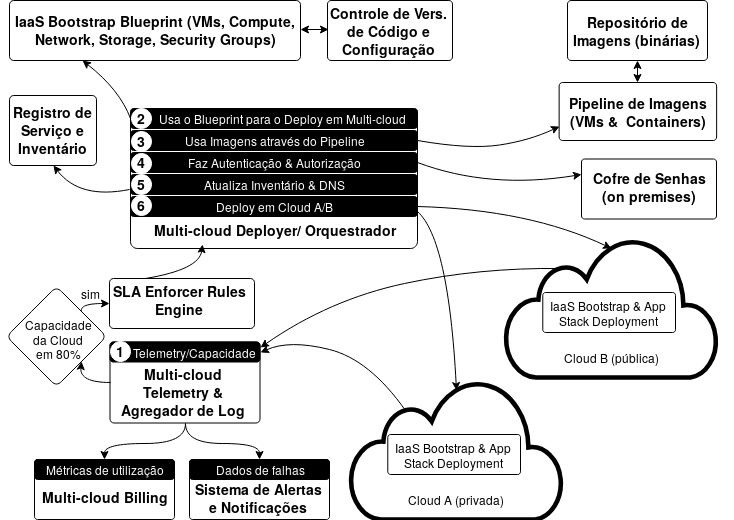
\includegraphics[width=0.9\linewidth]{figuras/Figure1.png}
			\caption{legenda longa figura1}
			\label{fig:figure1}
		\end{figure}

	O cenário descrito acima inicia em 1 - Telemetry, assim possibilitando situações automatizadas de orquestração dos recursos na Multi-cloud, entretanto, um humano também poderia iniciar esse processo, passando instruções diretamente ao box \textbf{Multi-cloud Deployer/Orquestrator}, porém, na Figura1 essa situação não é representada.  
	
	Os processos descritos acima e esquematizados na Figura1 podem ser bastante complexos e envolver outros subprocessos e também um conjunto diversificado de ferramentas e softwares. Como exemplo, exploremos em mais detalhes o \textbf{Pipeline de Imagens}:
	

	
	O objetivo do processo da Figura2 é prover imagens binárias de servidores que estão dentro dos padrões para rodar em qualquer Cloud IaaS que fazem parte da Multi-cloud.
	
	Este processo de criação padronizada de imagens pode alcançar seus objetivos utilizando produtos open-source. Os referenciados na Figura2 são; \textbf{Spinnaker} (http://www.spinnaker.io) que é uma plataforma para entrega contínua (\textit{Continuous Delivery}) de \textit{releases} de software em ambiente Multi-cloud. \textbf{Packer} (https://www.packer.io) é um framework capaz de produzir multiplas imagens em formatos diferentes, apropriadas para a maioria dor provedores de Cloud (Públicas e Privadas). Packer pode ser usado com uma variedade grande de \textit{build systems}, dentre os quais destacamos o \textbf{Jenkins} (https://jenkins.io).
	
	\underline{ver 829 e 2363}
	
		\begin{figure}[H]
			\centering
			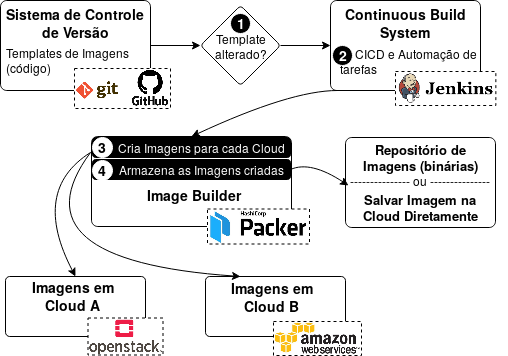
\includegraphics[width=0.7\linewidth]{figuras/Figure2.png}
			\caption{legenda longa figura2}
			\label{fig:figure2}
		\end{figure}
	
	O processo ilustrado na Figura2 é iniciado a partir de um \textit{commit} no \textbf{Sistema de Controle de Versão} em alguma \textit{branch} (Master por exemplo) que é monitorada pelo \textbf{Continuous Build System (1)}. Sempre que uma alteração é feita, o Jenkins executa as rotinas \textbf{(2)} que são requisitos para que o Packer (principal software do \textbf{Image Builder}) possa gerar as imagens de acordo com os \textit{blueprints} de cada Cloud \textbf{(3)}. O Packer pode armazenar essas imagens para uso futuro em um repositório centralizado (\textit{on-premises} geralmente) ou pode também gravar cada imagem na respectiva Cloud \textbf{(4)}, essa última alternativa pode ser mais rápida na hora de criar uma instância, pois não precisa fazer a transferência (via Internet) da Imagem armazenada on-premises para a Cloud.
	
	\section{Validação Experimental - Application Deployment in Multi-Cloud Environment}
	
	Uma das maneiras de experimentar o processo de deploy de IaaS e PaaS em Multi-cloud pode ser feito através do uso de alguns softwares que automatizam a criação de recursos em Cloud. O uso das consoles WEB ou SDKs disponibolizadas pelos principais provedores de Cloud propicia maior chance de erro humano, requer que a documentação seja feita adicionalmente e não aproveita os benefícios da Infraestrutura como Código, discutida a seguir.  
	
	\subsection{Infraestrutura como Código com Terraform}
	
	Infraestrutura como código – IaC (Infrastructure as Code) é o processo de gerenciamento e provisionamento de recursos de infraestrutura através de código e arquivos de configuração que descrevem o estado desejado para os recursos de infraestrutura. IaC usa definições declarativas ao invés de processos manuais ou procedurais. Como se tratam de arquivos de código, as definições podem ser armazenadas em um sistema de controle de versões, tal como o Git.
	
	Algumas vantagens da utilização de IaC incluem a \textbf{Eliminação de tarefas repetitivas} e possibilita \textbf{fácil replicação de implementações} quando o bloco de código pode ser executado repetidas vezes, fazendo poucas modificações (ou nenhuma em alguns casos) para criar ou modificar novos ambientes (Produção, Teste, Desenvoçvimento) ou implementar em Clouds diferentes (GCP, Azure ou AWS por exemplo). Uma vez que a infra está codificada de forma estruturada e geralmente em módulos, o código podee ser \textbf{Reaproveitado}. O fato da infraestrutura estar definida toda em código, e este estar \textbf{Versionado} em ferramentas como Git, possibilita \textbf{maior controle nas aplicações de mudança} nos ambientes possibilitando, inclusive, a \textbf{Recuperação de Desastres ou Disaster Recovery}. O versionamento do código em Git, também possibilita a simplificação da \textbf{Documentação do Código}, bem como sua \textbf{Manutenção e Suporte}. Além disso, com IaC, fica fácil utilizar-se das mesmas técnicas de \textbf{planejamento e testes automatizados} há muito utilizadas por desenvolvedores.
	
	
	https://www.hpe.com/br/pt/what-is/infrastructure-as-code.html	
	
	https://blog.marcelocavalcante.net/blog/2018/10/22/infraestrutura-como-codigo-com-terraform/
	

	Outro benefício importante deste esstud é a enfase em padrões "fault tolerant" que implicam na garantia que sistemas atinjam uptime e resiliencia à stress e falhas adequadas. 
	
	Implementação Open-source da plataforma com padrão neutro (vendor-neutral) será desenvolvida/apresentada para validar padrões e guias de adoção. Usaremos open-source software para demonstrar como os padrõe podem ser impleentados fazem este estudo mais util/completo/específico que padrões enéricos como os descrito em http://www.cloudpatterns.org.
	O resultado deste estudo será um catálogo de Padrões de Cloud "Fault Tolerant", Seguro e de alta performance com as soluções mapeadas com software open-source com exemplos do deploy (e alguns templates/pseudo-codigo) que podem ser usados para implementar um stack completo de infraestrutura que será compativel com a especificação OASIS CAMP (Cloud Application Management for Platforms) e mais tarde, com OASIS TOSCA (Topology and Orchestration Specification for Cloud Applications).
	
	Em seguida, todos os padrões serão validados usando software Open Source. A maioria das ofertas em cloud não seria possível sem uso de software open source (e.g. hypervisors Xen e KVM). Como selecionamos os melhores projetos open-source? We need to selec the projects with a large and active community, quantos "commiters" estão ativos, quantos contribuidores são de diferentes organizações ou este é um projeto open-source de uma única empresa (algumas empresas desenvolvem open-source software mas não aceitam contribuições externas - Read Only Opensource). Idealmente, melhor ainda se a solução open-source tiver alguma empresa mantenedora/responsável por oferecer serviços de consultoria e bug-fixes (caso a empresa não tenha todo o expertise in-house). 
	
	\section{Conclusion}
		
	Conclusão ...
	
	% \textbf{Texto negrito}. Seleciona e CTRL + b
	% \textit{Text itálico}. Seleciona e ctrl + i
	% \textbf{\textit{Text negrito e itálico}}
	% \underline{Text undeline} 
	
	% \begin{flushleft}
	%	Texto à esquerda
	% \end{flushleft}
	
	% \begin{center}
	%	Texto centralizado.
	% \end{center}
	
	% \begin{flushright}
	%	Texto à direita.
	% \end{flushright}
	
	% {\tiny Texto pequeno.}
	% {\LARGE Texto Grande.}
	% Texto Normal.
	
	% \part[test]{title}
	
	% \colorbox{gray}{\textcolor{green}{fundo em cinza com texto verde}}
	% \pagecolor{blue}
	
	\cite{Ferrer:2012}
	\cite{Bond:2015}
	\cite{Morris:2016}
	\cite{Fisher:2018}
	
	\nocite{Bond:2015}
	
	\newpage
	%\bibliographystyle{alpha}
	%\bibliographystyle{plain}
	%\bibliographystyle{unsrt}
	%\bibliographystyle{abbrv}
	%\bibliographystyle{apalike}
	\bibliographystyle{sbc}	
	\bibliography{artigo_multicloud.bib}
	
\end{document}
